\begin{frame}
	\frametitle{Sun Myung Park: Coupled neutronics/thermal-hydraulics analysis}
		\begin{columns}
		\column[t]{6cm}
		My current research interests:
		\begin{block}{Moltres}
			\begin{itemize}
				\item Developing and improving capabilities in Moltres \\
				\item Currently working on
				implementing the k-$\epsilon$ turbulence model in Moltres.
			\end{itemize}
		\end{block}
		\begin{block}{\gls{MSFR}}
			\begin{itemize}
			\item Performing safety analyses of the \gls{MSFR} for various
			accident transients using Moltres with the k-$\epsilon$ model to
			include turbulence effects
			\end{itemize}
		\end{block}
		\column[t]{4cm}
		\begin{figure}[htbp!]
			\begin{center}
				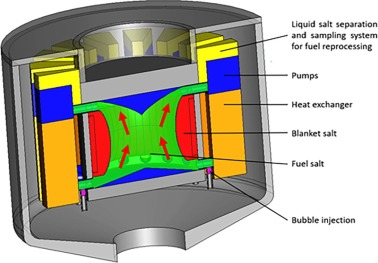
\includegraphics[height=3cm]{./images/msfr}
			\end{center}
			\caption{Schematic diagram of the \gls{MSFR}}
			\label{fig:msfr}
		\end{figure}
		\end{columns}
\end{frame}

\begin{frame}
	\frametitle{Sun Myung Park}
		\begin{columns}
			\column[t]{.5\textwidth}
			\begin{figure}[htbp!]
				\centering
				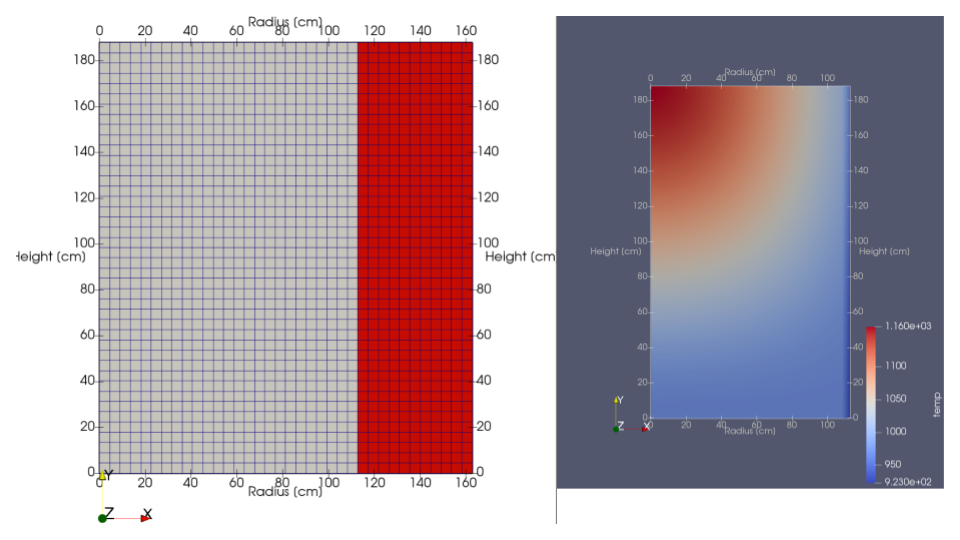
\includegraphics[height=2.8cm]{./images/mesh}
      			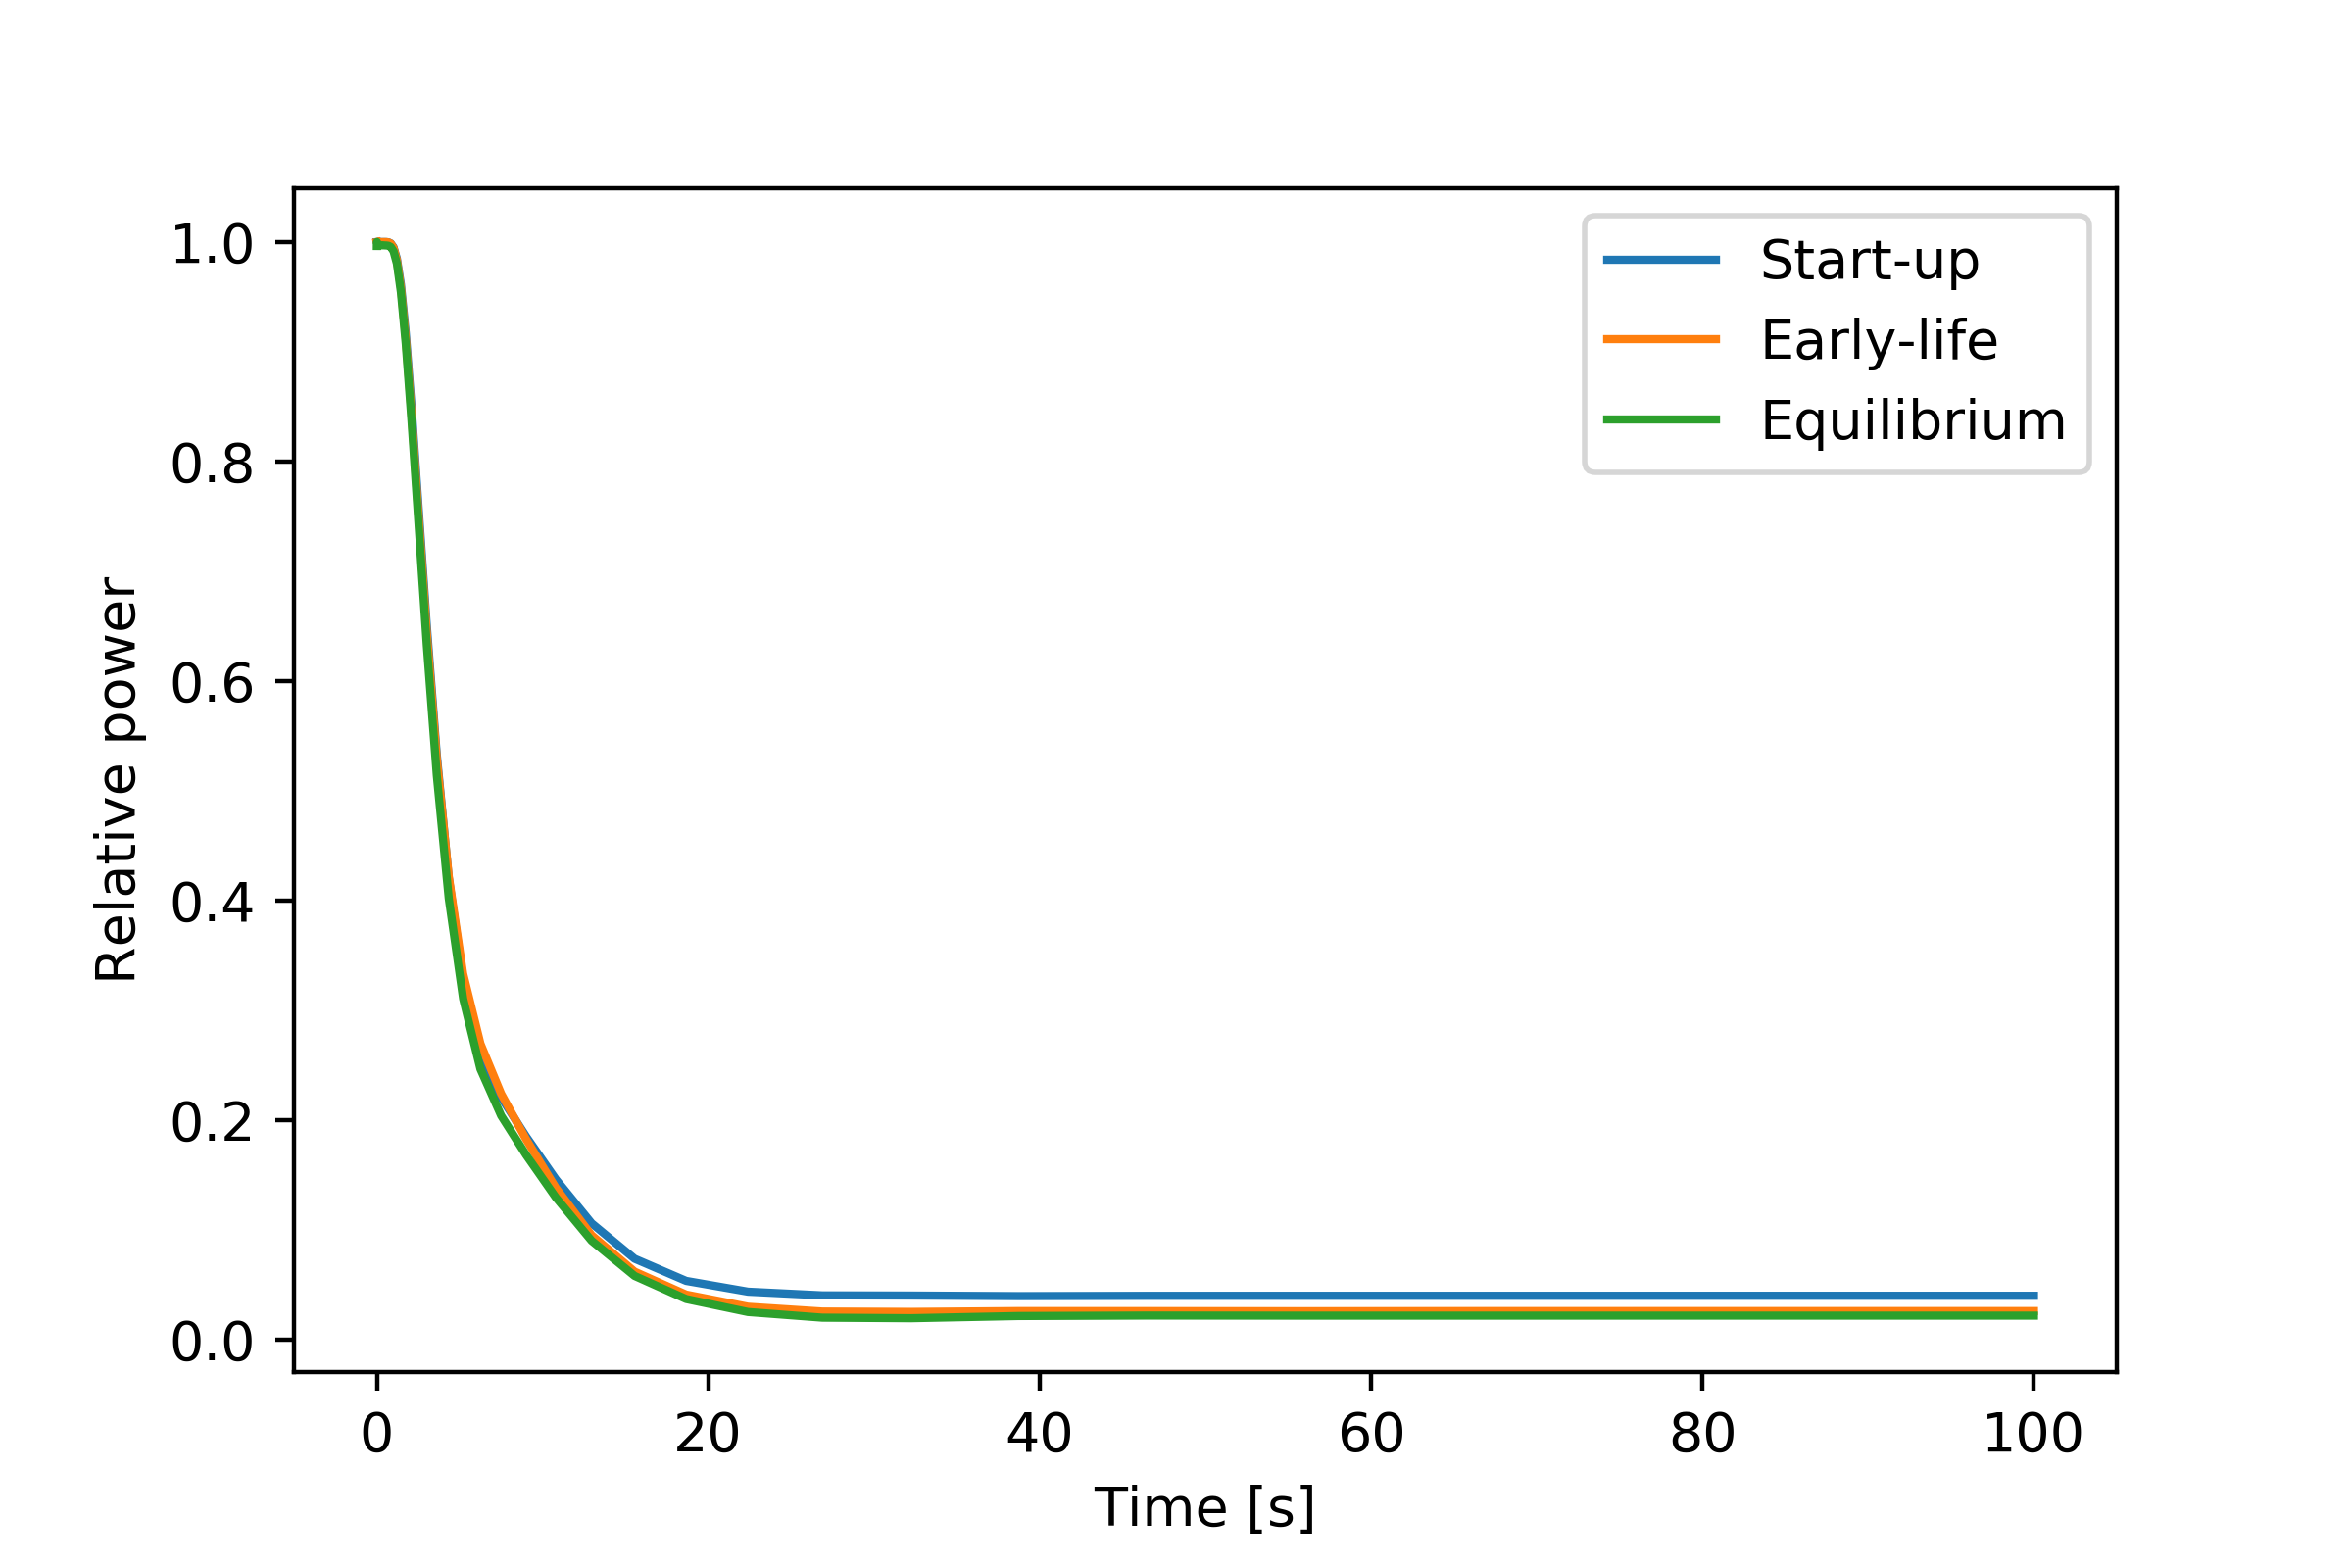
\includegraphics[height=2.8cm]{./images/loscaheat}
    			\caption{\scriptsize Clockwise from top left: MSFR 2D
    			axisymmetric mesh, steady state fuel temperature distribution,
    			relative power during a loss of heat sink scenario.}
			\end{figure}
			\vspace{.1cm}
			\column[t]{.5\textwidth}
			\begin{figure}
				\centering
				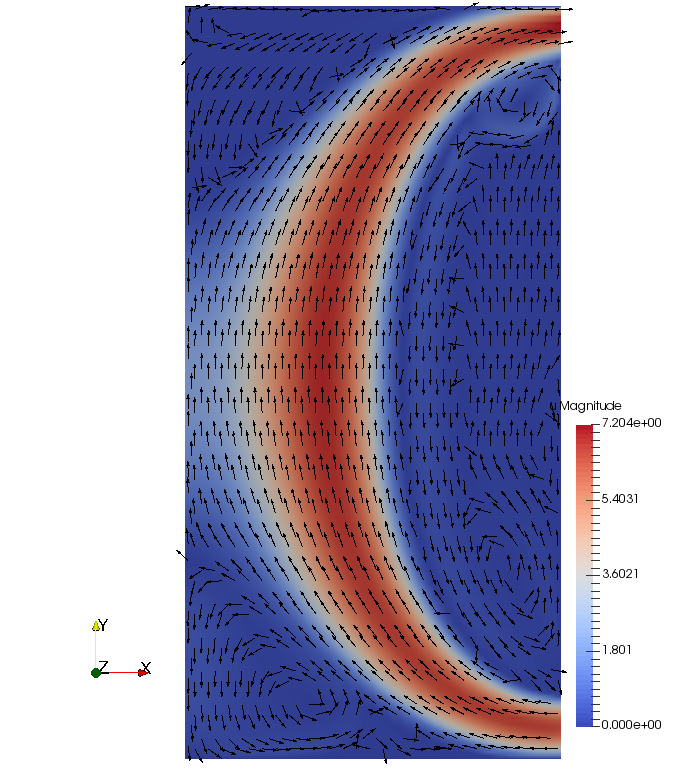
\includegraphics[width=.9\textwidth]{./images/ins-flow}
				\caption{\footnotesize Velocity distribution produced from the
				incompressible Navier-Stokes equations}
			\end{figure}
		\end{columns}
\end{frame}